\chapter{Jailhouse y Xen en UltraZed}

\section{Jailhouse}
Como se ha expuesto anteriormente, la denominación de Jailhouse es la de un \textit{hipervisor de particionamiento basado en Linux} \cite{jailhouse_github}. Es capaz de ejecutar programas baremetal junto con sistemas operativos guest y siempre partiendo desde Linux. Con este propósito, empleando las extensiones de virtualización del microprocesador en cuestión, configura una serie de celdas que no pueden interferirse entre ellas.\\
Una vez que Jailhouse está activado, toma el control absoluto del harwdare que tiene debajo. Necesita de un sistema operativo Linux que lo cargue y sus herramientas de control de celdas están basadas también en Linux.

\subsection{Compilación de Jailhouse}
El código fuente del proyecto Jailhouse está alojado en \cite{jailhouse_github}. En el momento de la elaboración del presente documento la versión en curso es la 0.11.\\
Desde el punto de vista de Linux, Jailhouse es un módulo del kernel (extensión .ko). En el momento que se carga el módulo, Jailhouse inserta el firmware del propio hipervisor en una zona de memoria reservada en arranque y crea el dispositivo \textit{/dev/jailhouse} en el sistema. Este dispositivo es el que utilizan las herramientas de gestión de Jailhouse que se ejecutan desde Linux para interactuar con el hipervisor y crear, arrancar, parar y destruir los sistemas guest o celdas.\\

El proceso de creación del propio módulo de Jailhouse necesita una serie de herramientas de compilación cruzada para la arquitectura de la plataforma que se está utilizando y también necesita el código fuente del kernel de Linux en el que se va a instalar como módulo.\\
En el anexo \ref{petalinux} se detalla el proceso de configuración y generación de un proyecto PetaLinux basado en la plataforma anteriormente descrita. Petalinux proporciona el compilador, linker, etc. necesarios a la hora de generar software para la arquitectura ARMv8 y el proceso de construcción del proyecto requiere del código fuente del kernel a fin de generar la imagen que de ejecutará en la tajeta Ultrazed\texttrademark.\\

Con todos estos elementos, lo único que hay que hacer para compilar Jailhouse para la arquitectura destino y el kernel de Linux generado con PetaLinux es ejecutar los siguientes commandos el la \textit{shell}

\begin{lstlisting}[style=CStyle]
  $ git clone git@github.com:siemens/jailhouse.git
  $ cd jailhouse
  $ export ARCH=arm64
  $ export CROSS_COMPILE=aarch64-linux-gnu-
  $ make KDIR=~/workspace/ehu-upv/linux-xlnx-xilinx-v2018.3/
\end{lstlisting}

Al final de este proceso, si todo ha ido bien, se habrá generado el módulo del kernel \textit{jailhouse.ko}.

\begin{lstlisting}[style=CStyle]
...
Building modules, stage 2.
  MODPOST 1 modules
  CC      /home/alex/workspace/ehu-upv/jailhouse/driver/jailhouse.mod.o
  LD [M]  /home/alex/workspace/ehu-upv/jailhouse/driver/jailhouse.ko
\end{lstlisting}

\subsection{Configuración de celdas}

Las celdas en Jailhouse se definen mediante una serie de ficheros \textit{.c} que se encuentran en la carpeta \textit{configs}. En esta localización aparen las carpetas correspondientes a las arquitecturas de microprocesadores soportadas por Jailhouse.

\begin{lstlisting}[style=CStyle]
$ ls -la
total 32
drwxrwxr-x  5 alex alex  4096 Jun  9 21:27 .
drwxrwxr-x 14 alex alex  4096 Jul 21 20:49 ..
drwxrwxr-x  3 alex alex  4096 Jun 23 12:59 arm
drwxrwxr-x  3 alex alex 12288 Jul 21 19:06 arm64
-rw-rw-r--  1 alex alex  1038 Jun  9 21:26 Makefile
-rw-rw-r--  1 alex alex     0 Jul 21 20:49 modules.order
drwxrwxr-x  2 alex alex  4096 Jun 29 20:03 x86
\end{lstlisting}

Para cada arquitectura existe un fichero \textit{.c} por cada celda del sistema. La celda Linux llamada \textit{root cell} siempre está presente y para cada caso de tarjeta existen diferentes celdas de referencia dependiendo de la aplicación. El resto de celdas reciben el nombre de \textit{inmate}. Si para una tarjeta en concreto existe la celda Linux y otras dos celdas \textit{inmate}, aparecerán tres ficheros; cada uno con la definición de una celda. Por ejemplo para la tarjeta Ultra96 (\url{https://www.96boards.org/product/ultra96/}) existen los siguientes ficheros:

\begin{lstlisting}[style=CStyle]
alex@xubuntu16:~/workspace/ehu-upv/jailhouse/configs$ ls -la arm64/ultra96*
-rw-rw-r-- 1 alex alex 2661 Jul 21 17:30 arm64/ultra96.c
-rw-rw-r-- 1 alex alex 1665 Jul 21 17:30 arm64/ultra96-gic-demo.c
-rw-rw-r-- 1 alex alex 2745 Jul 21 17:30 arm64/ultra96-linux-demo.c
\end{lstlisting}

Al compilar Jailhouse se genera un fichero con extensión \textit{.cell} por cada \textit{.c}. Los ficheros \textit{.cell} son los que utiliza la herramienta de gestión de sistemas guest desde la celda Linux.\\
En el momento de elaborar el presente TFM la tarjeta UltraZed\texttrademark no estaba entre la lista de plataformas soportadas y probadas de Jailhouse por lo que no existía ningún fichero de celda para la misma. Como ya se ha comentado anteriormente, al incluir un chip de la misma familia que la tarjeta Xilinx ZCU102 y la Ultra96, se consideró que la adaptación sería posible por lo que se han creado los ficheros correspondientes a la \textit{root cell} y a la celda con la aplicación baremetal de la forma que se describe en los siguientes apartados.

\subsubsection{Celda Linux}

La celda de Linux o \textit{root cell} contiene la definición de lo que va a ser el sistema y de cómo se van a repartir los diferentes recursos. El fichero creado para la UltraZed\texttrademark \textit{ultrazed\_ehu.c} contiene la estructura \textit{config} que necesita Jailhouse a fin de localizar en el mapa de memoria los diferentes recursos de la plataforma.
\begin{lstlisting}[style=CStyle]
#include <jailhouse/types.h>
#include <jailhouse/cell-config.h>

#define ARRAY_SIZE(a) (sizeof(a) / sizeof(a[0]))

struct {
	struct jailhouse_system header;
	__u64 cpus[1];
	struct jailhouse_memory mem_regions[8];
	struct jailhouse_irqchip irqchips[1];
} __attribute__((packed)) config = {
	(...)
\end{lstlisting}

La estructura principal que define el sistema tiene los siguientes campos:
\begin{itemize}
  \item Cabecera: en este campo se especifican las direciones físicas de memoria de los componentes que necesita configurar Jailhouse. Todas estas direcciones corresponden al mapa de memoria del Zynq\textregistered UltraScale+\texttrademark MPSoC \cite{mpsoc_registers}.\\
  \begin{lstlisting}[style=CStyle]
  (...)
  .header = {
		.signature = JAILHOUSE_SYSTEM_SIGNATURE,
		.revision = JAILHOUSE_CONFIG_REVISION,
		.flags = JAILHOUSE_SYS_VIRTUAL_DEBUG_CONSOLE,
		.hypervisor_memory = {
			.phys_start = 0x40000000,
			.size =       0x01000000,
		},
		.debug_console = {
			.address = 0xff000000,
			.size = 0x1000,
      .type = JAILHOUSE_CON_TYPE_XUARTPS,
			.flags = JAILHOUSE_CON_ACCESS_MMIO |
				 JAILHOUSE_CON_REGDIST_4,
		},
		.platform_info = {
			.pci_mmconfig_base = 0xfc000000,
			.pci_mmconfig_end_bus = 0,
			.pci_is_virtual = 1,
			.pci_domain = -1,
			.arm = {
				.gic_version = 2,
				.gicd_base = 0xf9010000,
				.gicc_base = 0xf902f000,
				.gich_base = 0xf9040000,
				.gicv_base = 0xf906f000,
				.maintenance_irq = 25,
			},
		},
		.root_cell = {
			.name = "UltraZed SoM ehu",

			.cpu_set_size = sizeof(config.cpus),
			.num_memory_regions = ARRAY_SIZE(config.mem_regions),
			.num_irqchips = ARRAY_SIZE(config.irqchips),
			.vpci_irq_base = 136-32,
		},
    (...)
  \end{lstlisting}
  Por ejemplo aquí aparece la dirección en la que se va a alojar el propio hipervisor. En este ejemplo la dirección es la 0x40000000. Esta dirección ha de estar libre en el momento en el que Linux instale el módulo del kernel que carga el hipervisor justo por encima del hardware como se muestra en la figura \ref{fig:jail_2}. Esta dirección forma parte de la memoria \acrshort{DDR} \acrshort{RAM} y a fin de garantizar que está libre cuando arranca la \textit{root cell} Linux lo que se hace es modificar los parámetros con los que el cargador de arranque U-Boot lanza el kernel, lo que se conoce como \textit{kernel command line}. En el \textit{device-tree} se puede definir el tamaño al que se le da acceso a Linux mediante el parámetro ``mem'' dentro de ``bootargs''.
  \begin{lstlisting}[style=CStyle]
  chosen {
		bootargs = "earlycon console=ttyPS0,115200 clk_ignore_unused earlyprintk mem=1024M";
		stdout-path = "serial0:115200n8";
	       };
  \end{lstlisting}
  Al proporcionar 1 de los 2 GB de memoria \acrshort{DDR} \acrshort{RAM} al kernel de linux el mapa de memoria al que puede acceder va desde la dirección 0x00000000 a la 0x3FFFFFFF. De este modo la dirección 0x40000000 está libre para el hipervisor.\\
  En la cabecera también se indica cual es la \acrshort{UART} por la que imprimir los mensajes de debug de la \textit{root cell} indicando la dirección de memoria del periférico.
  Otra información importante que aparece en la cabecera son las direcciones referentes al controlador de interrupciones que como se puede observar empieza en la dirección 0xF9010000 \cite{mpsoc_registers}. Jailhouse necesita conocer la ubicación del \acrshort{GIC} para configurarlo y ser capaz de virtualizar interrupciones y direccionarlas a la celda que corresponda.

  \item Número de CPUs: en el parámetro \textit{cpus} se indica mediante flags los núcleos de los que dispone la celda.
  \begin{lstlisting}[style=CStyle]
  (...)
  .cpus = {
		0xf,
	},
  (...)
  \end{lstlisting}
  En el caso de la \textit{root cell} se puede ver que en principio los 4 núcleos Cortex-A53 del MPSoC están al servicio de la celda.

  \item Zonas de memoria: En esta parte de la configuración de la celda se especifican las zona de memoria de las que tiene que ser consciente.
  \begin{lstlisting}[style=CStyle]
  (...)
  .mem_regions = {
		/* MMIO (permissive) */ {
			.phys_start = 0xfd000000,
			.virt_start = 0xfd000000,
			.size =	      0x03000000,
			.flags = JAILHOUSE_MEM_READ | JAILHOUSE_MEM_WRITE |
				JAILHOUSE_MEM_IO,
		},
		/* RAM */ {
			.phys_start = 0x0,
			.virt_start = 0x0,
			.size = 0x40000000,
			.flags = JAILHOUSE_MEM_READ | JAILHOUSE_MEM_WRITE |
				JAILHOUSE_MEM_EXECUTE,
		},
		/* RAM */ {
			.phys_start = 0x42000000,
			.virt_start = 0x42000000,
			.size = 0x3e000000,
			.flags = JAILHOUSE_MEM_READ | JAILHOUSE_MEM_WRITE |
				JAILHOUSE_MEM_EXECUTE,
		},
		/* PL gpio switches */ {
			.phys_start = 0xA0000000,
			.virt_start = 0xA0000000,
			.size = 0x00001000,
			.flags = JAILHOUSE_MEM_READ | JAILHOUSE_MEM_WRITE |
				JAILHOUSE_MEM_IO,
		},
		/* PL gpio leds */ {
			.phys_start = 0xA0001000,
			.virt_start = 0xA0001000,
			.size = 0x00001000,
			.flags = JAILHOUSE_MEM_READ | JAILHOUSE_MEM_WRITE |
				JAILHOUSE_MEM_IO,
		},
  (...)
  \end{lstlisting}
  Aparecen por ejemplo los periféricos de la zona de \acrshort{PL} que están mapeados en memoria al estar conectados mediante el bus \acrshort{AXI}. También las zonas de \acrshort{RAM} que no están ocupadas por el hipervisor.

  \item Interrupciones: en el campo \textit{irqchips} se definen las interrupciones que va manejar la celda en cuestion.
  \begin{lstlisting}[style=CStyle]
  (...)
  .irqchips = {
		/* GIC */ {
			.address = 0xf9010000,
			.pin_base = 32,
			.pin_bitmap = {
				0xffffffff, 0xffffffff, 0xffffffff, 0xffffffff,
			},
		},
	},
  (...)
  \end{lstlisting}
  Más concretamente en el campo \textit{pin\_bitmap} aparecen cuáles de las 128 fuentes de interrupción que se pueden manejar.

\end{itemize}

\subsubsection{Celda baremetal} \label{jailhouse:baremetal}
Lo único que se necesita definir en la celda \textit{inmate} que aloja la aplicación baremetal es el núcleo o núcleos en los que va a desplegarse, las zonas de memoria que se van a asignar y las interrupciones que se van a manejar. A grandes rasgos estas tres definiciones aparecen de la siguiente forma en el fichero \textit{ultrazed\_ehu\_irq.c}:

\begin{lstlisting}[style=CStyle]
(...)
.cell = {
		.signature = JAILHOUSE_CELL_DESC_SIGNATURE,
		.revision = JAILHOUSE_CONFIG_REVISION,
		.name = "gpio-leds-demo",
		.flags = JAILHOUSE_CELL_PASSIVE_COMMREG,

		.cpu_set_size = sizeof(config.cpus),
		.num_memory_regions = ARRAY_SIZE(config.mem_regions),
		.num_irqchips = ARRAY_SIZE(config.irqchips),
		.pio_bitmap_size = 0,
		.num_pci_devices = 0,

		.console = {
			.address = 0xff010000,
			.type = JAILHOUSE_CON_TYPE_XUARTPS,
			.flags = JAILHOUSE_CON_ACCESS_MMIO |
				 JAILHOUSE_CON_REGDIST_4,
		},
	},
(...)
.cpus = {
		0x8,
	},
(...)
/* UART */ {
    .phys_start = 0xff010000,
    .virt_start = 0xff010000,
    .size = 0x1000,
    .flags = JAILHOUSE_MEM_READ | JAILHOUSE_MEM_WRITE |
      JAILHOUSE_MEM_IO | JAILHOUSE_MEM_ROOTSHARED,
  },
/* GPIO_SWITCHES */ {
    .phys_start = 0xA0000000,
    .virt_start = 0xA0000000,
    .size = 0x00001000,
    .flags = JAILHOUSE_MEM_READ | JAILHOUSE_MEM_WRITE |
      JAILHOUSE_MEM_IO | JAILHOUSE_MEM_ROOTSHARED,
  },
  /* GPIO_LEDS */ {
    .phys_start = 0xA0001000,
    .virt_start = 0xA0001000,
    .size = 0x00001000,
    .flags = JAILHOUSE_MEM_READ | JAILHOUSE_MEM_WRITE |
      JAILHOUSE_MEM_IO | JAILHOUSE_MEM_ROOTSHARED,
  },
(...)
.irqchips = {
		/* GIC */ {
			.address = 0xf9010000,
			.pin_base = 32,
			.pin_bitmap = {
				1 << (54 - 32),
				0,
				0,
				1 << (136 - 128)
			},
		},
	}
(...)
\end{lstlisting}

De estas secciones, cabe destacar la parte en la que se le asignan a la celda solo las regiones de memoria correspondientes a los periféricos de \acrshort{PL} y \acrshort{UART} que va a manejar el programa.\\
En cuanto a las interrupciones, en el campo \textit{pin\_bitmap} dentro de \textit{irqchips} solo se activan los flags correspondientes a las interupciones número 54 y 136, \acrshort{UART} 1 y \acrshort{PL}-\acrshort{PS} Grupo 1 interrupción 0 respectivamente \cite{mpsoc_registers}.\\
En el campo \textit{cpus} aparece el valor 0x8 (1000b) lo que indica que esta celda va a tener asignado el núcleo con identificador 3 (los identificador van de 0 a 3 para los 4 núcleos Cortex-A53).

\subsubsection{Aplicación baremetal} \label{app_baremetal}

Jailhouse proporciona una serie de funciones genéricas de configuración del sistema para poder ser utilizadas por las celdas \textit{inmates} en el directorio \textit{inmates/lib}. Aquí se encuentran por ejemplo la API para configurar el \acrshort{GIC}, Timer o \acrshort{UART}. Tomando como referencia el ejemplo existente para el manejo de la interrupción del temporizador privado de ARM (número 27) se ha desarrollado la aplicación que responde a la interupción 136 producida por un cambio en los valores del switch conectado a \acrshort{PL} descrito en la sección \ref{vivado_config}.

En el código resultante se inicializan los dispositivos que se van a utilizar en el bucle principal y se atiene a la interrupción en la función \textit{handle\_IRQ}:
\begin{lstlisting}[style=CStyle]
#include <inmate.h>
#include <gic.h>

#define GPIO_IRQ_NUM		136

(...)

static void handle_IRQ(unsigned int irqn)
{
    unsigned int taux = 0;
    /* gpio to 1  to capture event */
    mmio_write32((p_gpio_capture + 0/4), 0x1);

    /* Clear channel 1 interrupts */
    mmio_write32((p_gpio_switch + 0x120/4), 0x1);

    /* Get timer valuer from capture events */
    t1 = mmio_read32(p_capture_timer_0 + XTC_TLR_OFFSET/4);
    t2 = mmio_read32(p_capture_timer_1 + XTC_TLR_OFFSET/4);
    taux = t2 - t1;

    /* gpio to 0 again */
    mmio_write32((p_gpio_capture + 0/4), 0x0);
    printk("delay %u\n", taux);
    capture_timer_reload();
}

(...)
void inmate_main(void)
{
    printk("Jailhouse IRQ lattency test ...\n");

    map_range((void *)PL_DEVICES_BASE_ADDRESS, 0x5000, MAP_UNCACHED);
    mmio_write32((p_gpio_capture + 0/4), 0x0);

    capture_timer_init(); /* Initialize timer for lattency measurement */
    gpio_init_irq();      /* Initialize gpio irq axi_gpio_0 */
    pwm_timer_init();     /* Initialize timer for pwm output */

    /* Connect ISR handler to IRQ */
    gic_setup(handle_IRQ);
    gic_enable_irq(GPIO_IRQ_NUM);

    /* enable pwm output */
    pwm_timer_enable();

    halt();
}

\end{lstlisting}

\subsection{Test Linux + baremetal}

La tarjeta electrónica se va a arrancar con los artefactos generados en el proyecto de PetaLinux y descritos en el anexo \ref{petalinux}. En el caso de Jailhouse se requiere de una modificación extra en el \textit{device-tree} para deshabilitar en la celda Linux los dispositivos cuyo manejo corresponde a la celda con la aplicación baremetal. Como se ha descrito en la sección \ref{jailhouse_sota}, el hipervisor Jailhouse no permite que un periférico se utilice en más de una celda. Por defecto en el fichero \textit{pl.dtsi} que genera automáticamente PetaLinux basándose en el diseño implementado en \acrshort{PL} se crean los nodos de esos dispositivos para ser manejados desde Linux. En este caso no interesa que Linux maneje esos recursos por lo que se deshabilitan en el fichero \textit{system-user.dtsi} de la siguiente forma:
\begin{lstlisting}[style=CStyle]
&axi_gpio_0 {
  status = "disabled";
};
&axi_gpio_1 {
  status = "disabled";
};
&axi_gpio_3 {
  status = "disabled";
};
&axi_timer_0 {
  status = "disabled";
};
&axi_timer_1 {
  status = "disabled";
};
\end{lstlisting}

El primer paso para probar la respuesta de la aplicación baremetal descrita en la sección \ref{app_baremetal} es copiar en la plataforma destino los ficheros compilados de las definiones de celdas y el binario de la aplicación. En el caso de las celdas creadas para la tarjeta UltraZed\texttrademark son: \textit{ultrazed\_ehu.cell}, \textit{ultrazed\_ehu\_irq.cell} y \textit{irq\_demo.bin}.

\begin{lstlisting}[style=CStyle]
root@ultrazed_hyp_1:~# jailhouse enable ultrazed_ehu.cell

Initializing Jailhouse hypervisor v0.10 (106-g45d8346-dirty) on CPU 2
Code location: 0x0000ffffc0200800
Page pool usage after early setup: mem 45/4067, remap 0/131072
Initializing processors:
 CPU 2... OK
 CPU 1... OK
 CPU 3... OK
 CPU 0... OK
Initializing unit: irqchip
Initializing unit: PCI
Page pool usage after late setup: mem 65/4067, remap 5/131072
Activating hypervisor
[  496.674646] The Jailhouse is opening.
\end{lstlisting}

El commando \textit{jailhouse enbale} lo que hace es configurar la \textit{root cell} con la definición del fichero \textit{ultrazed\_ehu.cell}. En este momento lo que ocurre es que se carga el \textit{firmware} de Jailhouse en la dirección especificada para el hipervisor y a continuación crea una celda para alojar el sistema Linux que hasta ahora estaba ejecutándose de manera nativa. Esta \textit{root cell} a partir de este momento ya se ejecuta como un sistema guest. A partir de este momento la gestión de las celdas se realiza con la aplicación que se ejecuta en espacio de usuario de la \textit{root cell}. Esta herramienta se comunica con el hipervisor a través de commandos \textit{ioctl()} hacia el dispositivo \textit{/dev/jailhouse} que se ha creado al insertar el módulo \textit{jailhouse.ko}.
Como se puede observar en un principio los 4 núcleos están destinados a la \textit{root cell} y se configuran las zonas de memoria y las interrupciones.\\

En el siguiente comando se crea la celda para alojar la aplicación baremetal:

\begin{lstlisting}[style=CStyle]
root@ultrazed_hyp_1:~# jailhouse cell create ultrazed_ehu_irq.cell
[  506.076718] CPU3: shutdown
[  506.079422] psci: CPU3 killed.
Created cell "gpio-irq-demo"
Page pool usage after cell creation: mem 80/4067, remap 5/131072
[  506.091124] Created Jailhouse cell "gpio-irq-demo"
\end{lstlisting}

Al haber asignado el núcleo con identificador 3 a la celda, Jailhouse lo que hace es quitarle ese recurso a la celda Linux que era la que lo mantenía hasta el momento. A su vez el hipervisor asigna las zonas de memoria e interrupciones definidas para la celda guest haciendo que desde ese momento no estén disponibles para ninguna celda más.\\

Con el objetivo de cargar en memoria asignada a la celda la propia aplicación, se ejecuat el siguiente comando.
\begin{lstlisting}[style=CStyle]
root@ultrazed_hyp_1:~# jailhouse cell load 1 irqbutton_demo.bin
Cell "gpio-irq-demo" can be loaded
\end{lstlisting}

El último de los comandos es el que lanza la ejecución del la aplicación baremetal:
\begin{lstlisting}[style=CStyle]
root@ultrazed_hyp_1:~# jailhouse cell start 1
Started cell "gpio-irq-demo"
\end{lstlisting}

Este proceso es el que aparece representado a nivel de bloques en la figura \ref{fig:jail_2}.\\

En el caso de la aplicación desarrollada, simplemente se atienden a las interrupciones producidas por un bloque \acrshort{AXI} \acrshort{GPIO}, se mide la latencia mediante un temporizador y se muestra en pantalla. La salida de mensajes de la celda baremetal se produce por la \acrshort{UART}1, que es distinta a la que utilza la \textit{root cell}.

\begin{lstlisting}[style=CStyle]
Jailhouse IRQ lattency test ...

delay 96
delay 95
delay 95
(...)
\end{lstlisting}

Jailhouse incorpora una serie de comandos para el control de las celdas \textit{inmate}. Por ejemplo, mediante el siguiente comando se pueden listar las celdas activas del sistema:

\begin{lstlisting}[style=CStyle]
root@ultrazed_hyp_1:~/jailhouse# jailhouse cell list
ID      Name                    State             Assigned CPUs           Failed CPUs
0       UltraZed SoM ehu        running           0-2
1       gpio-irq-demo           running           3
\end{lstlisting}

\section{Xen}

Xen es el hipervisor que Xilinx tiene integrado en su herramientas de desarrollo y para el que da soporte. Al igual que Jailhouse, Xen también es un hipervisor de tipo 1 que una vez arrancado toma el control del hardware. Requiere de un dominio llamado Dom0 con privilegios especiales con la capacidad de acceder al hardware, manejar operaciones de entra y salida e interactuar con los demás dominios. También expone una interfaz de control con la que gestionar la creación, eliminación, inicio y parada de sistemas guest.


\subsection{Compilación de Xen} \label{xen_compilacion}

El código fuente de Xen se encuentra alojado oficialmente en \cite{xen_source}. Xilinx, al igual que hace con el kernel de Linux y con el cargador de arramque U-Boot, mantiene un repositorio público separado donde controla la versión de Xen que acompaña cada lanzamiento oficial de sus herramientas \cite{xen_source_xilinx}. La versión de Xen liberada con PetaLinux 2018.3 es la 4.11.\\
La generación de los artefactos de Xen está incluida en el proceso de PetaLinux, pero no está habilitada por defecto. Para ello, se deben ejecutar los siguientes comandos:\\
Seleccionar Xen dentro dentro del grupo de paquetes a incluir en el sistema de ficheros.
\begin{lstlisting}[style=CStyle]
$ petalinux-config -c rootfs
\end{lstlisting}

En el menú que se despliega al ejecutar el comando anterior, navegar hasta la ventana que se muestra en la figura \ref{fig:xen_menuconfig_1} y seleccionar la primera opción:
\begin{lstlisting}[style=CStyle]
Petalinux Package Groups  ---> packagegroup-petalinux-xen   --->  [*] packagegroup-petalinux-xen
\end{lstlisting}

\begin{figure*}[!h]
  \centering
  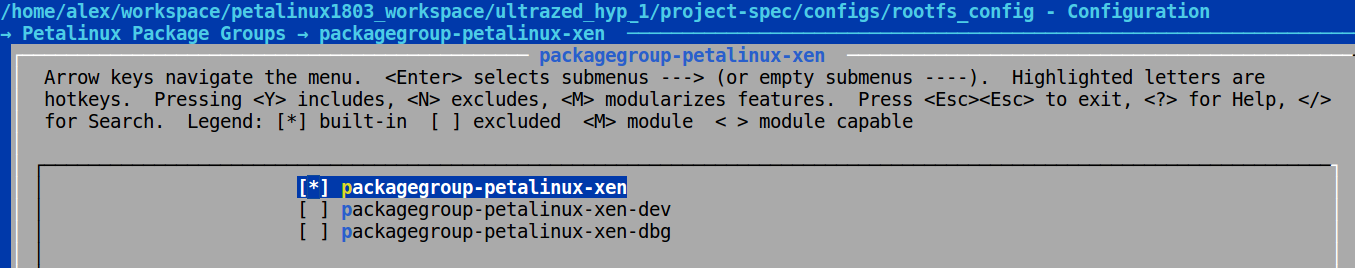
\includegraphics[width=1.0\textwidth]{recursos/petalinux_xen_1.png}
  \caption{Configuración de paquetes en el sistema de ficheros}
  \label{fig:xen_menuconfig_1}
\end{figure*}

Una vez se ha habilitada esta opción, guardar la configuración y salir. Es necesario reconstruir el proyecto con el comando:
\begin{lstlisting}[style=CStyle]
$ petalinux-buid
\end{lstlisting}

Al finalizar el proceso, entre los artefactos generados se encuentra el firmware de Xen que va a ser utilizado durante el arranque del sistema como se verá posteriormente. El nombre del fichero es \textit{xen.ub}

Alternativamente a la generación mediante PetaLinux, existe siempre la posibilidad de descargar el código fuente y compilarlo. Para ello, se deben ejecutar los siguientes comandos \cite{xen_source_xilinx}

\begin{lstlisting}[style=CStyle]
$ git clone git@github.com:Xilinx/xen.git
$ cd xen
$ make dist-xen XEN_TARGET_ARCH=arm64 CROSS_COMPILE=aarch64-linux-gnu-
$ mkimage -A arm -C none -T kernel -a 0x0200000 -e 0x00200000 -n Xen -d xen/xen  xen.ub
\end{lstlisting}

\subsection{Configuración de dominios}
\subsubsection{Dom0 Linux} \label{xen_dom0_config}

El Dom0 Linux que se va utilizar es prácticamente el mismo que se ejecutaría nativamente con los artefactos generados con PetaLinux. Únicamente mediante unos nodos en el \textit{device-tree}, se definen los parámetros necesarios para arrancar Xen y Linux como Dom0. Estos parámetros se recogen en un fichero \textit{xen.dtsi} que es necesario incluir. Dentro del proyecto PetaLinux, el fichero \textit{project-spec/meta-user/recipes-bsp/device-tree/files/system-user.dtsi} debe contener lo siguiente en el inicio:

\begin{lstlisting}[style=CStyle]
/include/ "system-conf.dtsi"
/include/ "xen.dtsi"
/ {
(...)
\end{lstlisting}

Es necesario también actualizar la receta de construcción del \textit{device-tree} en el proyecto de PetaLinux a fin de indicar la localización del fichero \textit{xen.dtsi}. Para ello, el fichero \textit{project-spec/meta-user/recipes-bsp/device-tree/device-tree.bbappend} debe contener las siguientes líneas:

\begin{lstlisting}[style=CStyle]
FILESEXTRAPATHS_prepend := "${THISDIR}/files:"

SRC_URI += "file://system-user.dtsi"
SRC_URI += "file://xen.dtsi"
\end{lstlisting}

El contenido del fichero \textit{xen.dtsi} es lo que utiliza Xen y el Dom0 para determinar la configuración con la que se arranca. En dicho fichero aparecen secciones como la siguiente:

\begin{lstlisting}[style=CStyle]
{
	chosen {
		#address-cells = <2>;
		#size-cells = <1>;

		xen,xen-bootargs = "console=dtuart dtuart=serial0 dom0_mem=768M bootscrub=0 maxcpus=1 timer_slop=0";
		xen,dom0-bootargs = "console=hvc0 earlycon=xen earlyprintk=xen maxcpus=1 clk_ignore_unused";

		dom0 {
			compatible = "xen,linux-zimage", "xen,multiboot-module";
			reg = <0x0 0x80000 0x3100000>;
		};
	};

};
(...)
\end{lstlisting}

En el parámetro \textit{xen,xen-bootargs} se especifica el dispositivo físico para la consola, el tamaño de la memoria (768MB) que se concede al Dom0, así como el máximo de CPUs. En el siguiente parámetro, destinado al Dom0, se define la consola como \textit{hvc0}. Esto implica que la consola del Dom0 pasa a través de Xen siendo la misma para los dos. En la sección \ref{section:text_xen} se muestran los mensajes producidos en el inicio del sistema tanto por Xen como por el Dom0.\\
Se indica también el tipo de Dom0 que va a arrancar Xen. En este caso se trata de un kernel de Linux en formato zimage que se debe cargar en la dirección 0x80000 de memoria en el cargador de arranque U-Boot como se verá también en las siguientes secciones.

El siguiente bloque del fichero contiene la definición de los dispositivos que pueden ser maestros de la MMU. En Xen para ARMv8 se hace uso de la extensión de virtualización que permite los mapeos de memoria virtual a física en dos fases como se explica en \cite{armv8_stage2}. De esta forma, se le indica a Xen la lista de los dispositivos que son capaces de mover datos directamente a memoria \acrshort{RAM} para permitir ese flujo a la hora de configurar la \acrshort{SMMU}.

\begin{lstlisting}[style=CStyle]
(...)
&smmu {
	status = "okay";
	mmu-masters = < &gem0 0x874
			&gem1 0x875
			&gem2 0x876
			&gem3 0x877
			&dwc3_0 0x860
			&dwc3_1 0x861
			&qspi 0x873
			&lpd_dma_chan1 0x868
			&lpd_dma_chan2 0x869
			&lpd_dma_chan3 0x86a
(...)
\end{lstlisting}

Por último, aparecen los dispositivos existentes en el \textit{device-tree} que no van a ser manejados desde el Dom0 y que serán cedidos directamente a alguno de los DomU. En este caso, en el DomU se va a utilizar la \acrshort{UART}1 y los periféricos de \acrshort{GPIO} y temporizador incluidos en la parte de \acrshort{PL}.

\begin{lstlisting}[style=CStyle]
(...)
&uart1 {
       xen,passthrough = <0x1>;
};

&axi_gpio_0 {
       xen,passthrough = <0x1>;
};

&axi_timer_0 {
       xen,passthrough = <0x1>;
};
(...)
\end{lstlisting}

A fin de que la inclusión del fichero \textit{xen.dtsi} tenga efecto, se contruye el \textit{device-tree} de nuevo.

\begin{lstlisting}[style=CStyle]
$ petalinux-buid -c device-tree
\end{lstlisting}

El proceso de generación del \textit{device-tree} produce un fichero con extensión \textit{.dtb} que va a ser utilizado tanto por Xen como por el Dom0 durante el arranque.

\subsubsection{DomU baremetal}

Xen necista un fichero de configuración para la ejecutar dominios no privilegiados. En dicho fichero se indican los parámetros que definen el DomU. En este caso, la definición que se ha utilizado se muestra a continuacion:

\begin{lstlisting}[style=CStyle]
#Guest name
name = "DomU_baremetal_app"
# Kernel image to boot
kernel = "DomU_baremetal_app.bin"
# Kernel command line options - Allocate 8MB
memory = 8
# Number of VCPUS
vcpus = 1
# Pin to CPU 1
cpus = [1]
irqs = [ 54, 136 ]
iomem = [ "0xff010,1", "0xA0000,1", "0xA0001,1", "0xA0002,1", "0xA0003,1" "0xA0004,1" ]
\end{lstlisting}

Como se observa en las primeras líneas, es necesario especificar el nombre del fichero binario que contiene la aplicación así como el tamaño del espacio de memoria que se le asigna para su ejecución. En este caso la aplicación ocupa unos pocos kilobytes, así que los 8 MB reservados son suficientes. En los siguientes parámetros se indica el número de CPUs virtuales (\textit{vcpu}) con las que se inicia el DomU y si se asigna específicamente alguno de los nucleos (\textit{cpu}). Este último parámetro es opcional. Al haber definido \textit{vpcu} y \textit{cpu}, ambos con valor 1, implica que se mapea específicamente la \textit{vcpu} con identificador 0 al núcleo con identificador 1. Estos parámetros admiten múltimples combinaciones que quedan fuera del alcance del presente trabajo.\\
En cuanto a las interrupciones, al igual que en la celda \textit{inmate} de Jailhouse de la sección \ref{jailhouse:baremetal}, se le indica a Xen que las interrupciones con números 54 (\acrshort{UART}1) y 136 (\acrshort{PL} a \acrshort{PS} grupo 1) deben ser redirigidas a el DomU.\\
Por último, en \textit{iomem} se definen las zonas de memoria que va a manejar directamente el DomU. En este caso se trata de la propia \acrshort{UART}1, los bloques de \acrshort{GPIO} y temporizadores inlcuidos en \acrshort{PL}.

\subsubsection{Aplicación baremetal}

Mediante el entorno de desarrollo \acrshort{XSDK} de Xilinx se pueden crear aplicaciones baremetal para ser lanzadas como DomU en Xen \cite{xen_domU_xsdk}. Como se muestra en la figura \ref{fig:domU_xsdk_1}, a nivel de configuración, la única diferencia con una aplicación baremetal que no esté destinada a ejecutarse con un hipervisor por debajo, es la indicación de que debe lanzarse con el nivel de excepción EL1 (\textit{hypervisor guest: yes}).

\begin{figure*}[!h]
	\centering
	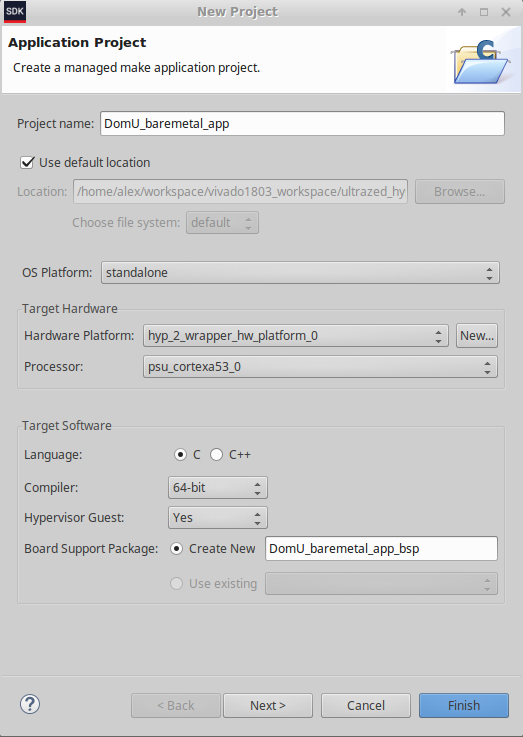
\includegraphics[width=0.70\textwidth]{recursos/domU_xsdk_1.png}
	\caption{Configuración de proyecto en XSDK}
	\label{fig:domU_xsdk_1}
\end{figure*}

Realmente, la opción de ejecutarse en EL1 tiene más implicaciones a nivel de software pero la herramienta de Xilinx abstrae de las mismas al desarrolador. Cuando se genera una aplicación en \acrshort{XSDK} se necesita un \acrshort{BSP}. En el caso de Xilinx, existen \acrshort{BSP}s que incluyen la inicialización a bajo nivel de los procesadores, así como los drivers de manejo de los dispositivos inluidos es las arquitecturas Zynq-7000 y MPSoC.\\
A la hora de crear una nueva aplicación, si no existe el correspondiente \acrshort{BSP}, la herramienta lo genera automáticamente. En un \acrshort{BSP}s generado para un DomU que va a ejecutarse sobre un hipervisor, se incluyen en el código las llamadas al hipervisor (\textit{hvc} en ARMv8) o \textit{hypercalls} mencionadas en el capítulo \ref{ch:introduccion:primera}.\\

La aplicación desarrollada está basada en uno de los ejemplos de Xilinx para manejo de interrupciones y sigue los mismos pasos que la celda \textit{inmate} de Jailhouse.
Primero habilita los temporizadores incluídos en la zona de \acrshort{PL}. Uno de ellos de utiliza para generar la señal \acrshort{PWM} que provoca las interrupciones del bloque \acrshort{GPIO} y el otro se configura para capturar los instantes en los que se produce la interrupción y el tiempo que se tarda en atenderla desde la correspondiente \acrshort{ISR}.

\begin{lstlisting}[style=CStyle]
(...)

/* Initialize the Capture Timer . If an error occurs then exit */
	Status = Tmr0_Init();
	if (Status != XST_SUCCESS) {
		return XST_FAILURE;
	}

	/* Initialize the PWM Timer . If an error occurs then exit */
	Status = Tmr1_Init(&TimerCounterInst, TMRCTR_DEVICE_ID);
	if (Status != XST_SUCCESS) {
		xil_printf("Tmrctr PWM Example Failed\r\n");
		return XST_FAILURE;
	}

(...)
\end{lstlisting}

A continuación se configura el controlador de interrupciones para capturar la interrupción con número 136:
\begin{lstlisting}[style=CStyle]
/* Enable the interrupt for the GPIO device.*/
	XScuGic_Enable(IntcInstancePtr, IntrId);

	/*
	 * Enable the GPIO channel interrupts so that push button can be
	 * detected and enable interrupts for the GPIO device
	 */
	XGpio_InterruptEnable(InstancePtr, IntrMask);
	XGpio_InterruptGlobalEnable(InstancePtr);
\end{lstlisting}

La \textit{ISR} para la interrupción 136 activa el \acrshort{GPIO} que provoca la captura en el temporizador con el siguiente bloque de código:
\begin{lstlisting}[style=CStyle]
void GpioHandler(void *CallbackRef)
{
  uint32_t *p_gpio_capture = (uint32_t *)XPAR_AXI_GPIO_3_BASEADDR;

	*p_gpio_capture = 0x1;

	IntrFlag = 1;

	/* Clear the Interrupt */
	XGpio_InterruptClear(&Gpio, GlobalIntrMask);

}
\end{lstlisting}

Por último, en el bucle principal del programa, se espera a que se active \textit{IntrFlag} para leer del temporizador de captura los valores correspondietes para calcular la latencia de la interuupción:

\begin{lstlisting}[style=CStyle]
(...)
while(irq_count < NUM_SAMPLES) {
		if (IntrFlag) {
			*p_gpio_capture = 0x0;
			IntrFlag = 0;
			irq_count++;

      /* Get capture timer values */
			t1[irq_count] = *(tmr_ptr_0 + XTC_TLR_OFFSET/4);
			t2[irq_count] = *(tmr_ptr_1 + XTC_TLR_OFFSET/4);
			Tmr0_reload();
		}
	}
(...)
\end{lstlisting}

Al compilar este código, la herramienta \acrshort{XSDK} genera el fichero \textit{DomU\_baremetal\_app.bin} que se utilizará en la tarjeta UltraZed\texttrademark durante el test de Xen.

\subsection{Test Dom0 Linux + DomU baremetal} \label{section:text_xen}

En el caso de Xen, la secuencia de arranque de la tarjeta electrónica difiere en el orden de los elementos respecto a Jailhouse. En este caso, el cargador de arranque U-Boot lanza directamente el firmware de Xen y desde aquí, se lanza el Dom0. Es necesario cargar en memoria, el binario de Xen generado en la sección \ref{xen_compilacion}, así como el \textit{device-tree} de la sección \ref{xen_dom0_config}, y la imagen del kernel de Linux del anexo \ref{petalinux}. Desde la consola de U-Boot, se situan los ficheros en las posiciones de memoria 0x1030000, 0x1000000 y 0x80000 respectivamente. Se pueden cargar los ficheros en esas posiciones ya sea por \acrshort{JTAG}, leyendo dede la tarjeta microSD o \acrshort{eMMC} o bien mediante tftp.
Con estos elementos se lanza el arranque de la siguiente forma desde la consola de U-Boot:

\begin{lstlisting}[style=CStyle]
(...)
In:    serial@ff000000
Out:   serial@ff000000
Err:   serial@ff000000
Board: Xilinx ZynqMP
Net:   ZYNQ GEM: ff0e0000, phyaddr 9, interface rgmii-id
eth0: ethernet@ff0e0000
Hit any key to stop autoboot:  0
ZynqMP>
ZynqMP> bootm 1030000 2000000 1000000
(...)
\end{lstlisting}

En el inicio del sistema, los mensajes que aparecen son del firmware de Xen:
\begin{lstlisting}[style=CStyle]
Starting kernel ...

 Xen 4.11.1-pre
(XEN) Xen version 4.11.1-pre (@) (aarch64-xilinx-linux-gcc (GCC) 7.3.0) debug=n  Mon Dec  3 21:50:14 UTC 2018
(XEN) Latest ChangeSet: Thu Nov 8 15:40:11 2018 -0800 git:b2edf52-dirty
(XEN) Processor: 410fd034: "ARM Limited", variant: 0x0, part 0xd03, rev 0x4
(XEN) 64-bit Execution:
(XEN)   Processor Features: 0000000000002222 0000000000000000
(XEN)     Exception Levels: EL3:64+32 EL2:64+32 EL1:64+32 EL0:64+32
(XEN)     Extensions: FloatingPoint AdvancedSIMD
(XEN)   Debug Features: 0000000010305106 0000000000000000
(XEN)   Auxiliary Features: 0000000000000000 0000000000000000
(XEN)   Memory Model Features: 0000000000001122 0000000000000000
(XEN)   ISA Features:  0000000000011120 0000000000000000
(XEN) 32-bit Execution:
(XEN)   Processor Features: 00000131:00011011
(XEN)     Instruction Sets: AArch32 A32 Thumb Thumb-2 Jazelle
(XEN)     Extensions: GenericTimer Security
(XEN)   Debug Features: 03010066
(XEN)   Auxiliary Features: 00000000
(XEN)   Memory Model Features: 10201105 40000000 01260000 02102211
(XEN)  ISA Features: 02101110 13112111 21232042 01112131 00011142 00011121
(XEN) Generic Timer IRQ: phys=30 hyp=26 virt=27 Freq: 99999 KHz
(XEN) GICv2 initialization:
(XEN)         gic_dist_addr=00000000f9010000
(XEN)         gic_cpu_addr=00000000f9020000
(XEN)         gic_hyp_addr=00000000f9040000
(XEN)         gic_vcpu_addr=00000000f9060000
(XEN)         gic_maintenance_irq=25
(XEN) GICv2: Adjusting CPU interface base to 0xf902f000
(XEN) GICv2: 192 lines, 4 cpus, secure (IID 0200143b).
(XEN) Using scheduler: SMP Credit Scheduler (credit)
(XEN) Allocated console ring of 16 KiB.
(XEN) Bringing up CPU1
(XEN) Bringing up CPU2
(XEN) Bringing up CPU3
(XEN) Brought up 4 CPUs
\end{lstlisting}

Una vez Xen ha arrancado, procecede a lanzar el Dom0, en este caso Linux, tal y como se ha indicado en la descripción del fichero \textit{xen.dtsi} en la sección \ref{xen_dom0_config}.\\
Una vez arrancado el Dom0, se copia el fichero de configuración del DomU (\textit{DomU.cfg}) y el fichero binario con la aplicación baremetal compilada con \acrshort{XSDK} (\textit{DomU\_baremetal\_app.bin}). Xen proporciona las herramientas de espacio de usuario necesarias para gestionar los dominios no privilegiados. Con objeto de lanzar el DomU, es necesario introducir el siguiente comando de \textit{shell}:

\begin{lstlisting}[style=CStyle]
root@ultrazed_hyp_1:~# xl create DomU.cfg
Parsing config from DomU.cfg
root@ultrazed_hyp_1:~#
\end{lstlisting}

En este momento, el la \acrshort{UART}1 empiezan a aparecer los mensajes de la aplicación baremetal del DomU, que tienen en siguiente aspecto:

\begin{lstlisting}[style=CStyle]
Xen IRQ Test ...
[1] t1 4999778 t2 4999562 taux 216
[2] t1 4999778 t2 4999560 taux 218
[3] t1 4999774 t2 4999558 taux 216
[4] t1 4999775 t2 4999560 taux 215
[5] t1 4999779 t2 4999562 taux 217
[6] t1 4999776 t2 4999559 taux 217
[7] t1 4999776 t2 4999560 taux 216
(...)
\end{lstlisting}

Xen, al igual que Jailhouse, dispone de una serie de comandos para gestionar los dominios no privilegiados desde el Dom0. Entre ellos se encuentra por ejemplo, el comando que lista los dominios que están activos en el sistema:

\begin{lstlisting}[style=CStyle]
root@ultrazed_hyp_1:~# xl list
Name                             ID   Mem VCPUs      State   Time(s)
Domain-0                          0   768     1     r-----      10.5
DomU                              1     8     1     r-----      62.3
\end{lstlisting}
